%--------------------------------------------------------------------
\medskip
\subsection{Si se utiliza ROLAP, se debe incluir un diseño modelo lógico}
\label{08}
Lo primero que se ha de hacer para realizar el diseño de un modelo lógico es identificar las dimensiones. Las \textbf{dimensiones} para este problema son: \texttt{Cliente}, \texttt{Proyecto}, \texttt{Auditor} y \texttt{Evaluación}. \\

Seguidamente, identificar los hechos. Los \textbf{hechos} son los resultados obtenidos en las encuestas. \\

Y por último, definir las métricas. Las \textbf{métricas} directas que se pueden definir son: 
\begin{itemize}
 \item \textit{Resultado final de la encuestas, cuya función de agregación sería la suma}.
 \item \textit{Encuesta con menor resultado, cuya función de agregación sería el mínimo}.
 \item \textit{Encuesta con mayor resultado, cuya función de agregación sería el máximo}. 
 \item \textit{Número total de encuestas, cuya función de agregación sería el conteo}. 
\end{itemize}

Una vez definidas las dimensiones, hechos y métricas, el siguiente paso es jerarquizar la información. Así pues, la jerarquización para todas las dimensiones anteriores es:
\begin{itemize}
 \item \texttt{Cliente}. Esta dimensión tiene dos jerarquías:
 \begin{itemize}
  \item \texttt{Local}, cuyos niveles son: \texttt{Código Local} y \texttt{Nombre Local}.
  \item \texttt{Localización}, cuyos niveles son: \texttt{Provincia} y \texttt{Oficina}. A su vez, el nivel de \texttt{Provincia}, tiene los siguientes niveles:
  \begin{itemize}
   \item \texttt{Población}.
   \item \texttt{Código Postal}.
  \end{itemize}

 \end{itemize}

 \item \texttt{Proyecto}. Esta dimensión solamente tiene la jerarquía \texttt{Proyecto} cuyo nivel es \texttt{Código Proyecto}.
 \item \texttt{Auditor}. Esta dimensión solamente tiene la jerarquía \texttt{Auditor} cuyo nivel es \texttt{Código Auditor}.
 \item \texttt{Evaluación}. Esta dimensión solamente tiene la jerarquía \texttt{Evaluación} con los siguientes niveles:
\begin{itemize}
 \item \texttt{Evaluación}.
 \item \texttt{Título}.
 \item \texttt{Fecha}.
\end{itemize}
\end{itemize}

Así pues, en la Figura \ref{08-image} se muestra el modelo lógico para el Data Mart Mistery Shopping.

\begin{figure}[!th]
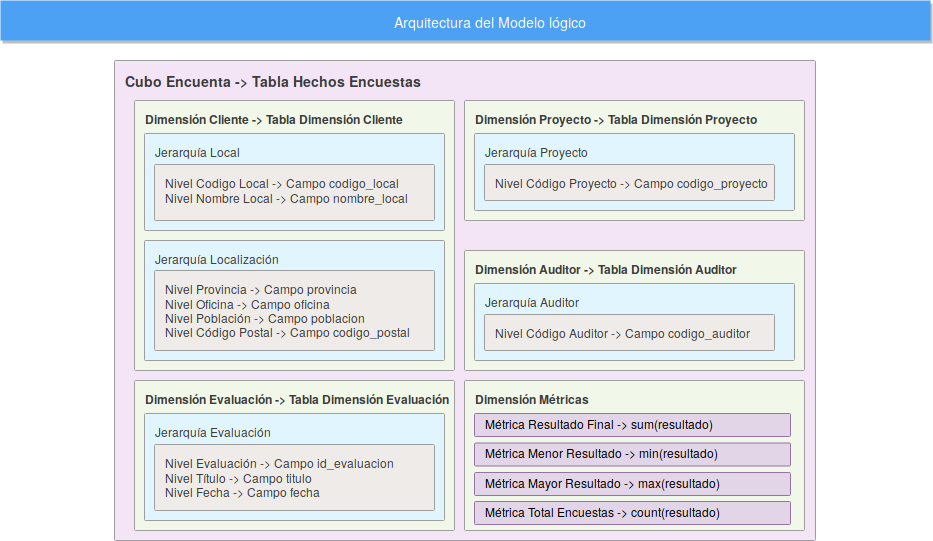
\includegraphics[scale=0.5]{08.png}
\centering
\caption{Modelo lógico para el Data Mart Mistery Shopping.}
\label{08-image}
\end{figure}

Partiendo del modelo en estrella de la Figura \ref{07-image}, la Figura \ref{08-1-image} muestra el modelo lógico con los identificadores y claves de cada una de las tablas.

\begin{figure}[!th]
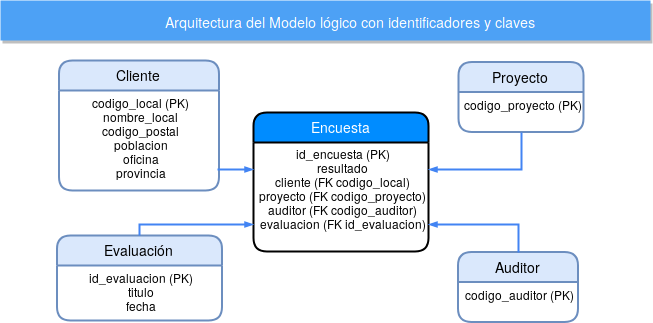
\includegraphics[scale=0.5]{08-1.png}
\centering
\caption{Modelo lógico con identificadores y claves para el Data Mart Mistery Shopping.}
\label{08-1-image}
\end{figure}
